\documentclass[preprint,12pt]{elsarticle}

\usepackage{amssymb}
\usepackage{amsmath}
\usepackage{graphicx}
\usepackage{booktabs}

%% TBD: confirm exact journal name for this special issue before submission
%% (special issue is hosted on ScienceDirect; "Utilities Policy" is our best
%% guess pending confirmation from the call for papers page).
\journal{Utilities Policy}

\begin{document}

\begin{frontmatter}

\title{Utility Planning and Water and Sanitation Tariff Burdens in Brazil: A Three-Decade Municipal Panel and Conditional Scenarios to 2033}

%% AUTHOR INFORMATION PENDING -- fill in real name(s), affiliation(s) and
%% corresponding email before submission. Do not submit with placeholders.
\author[label1]{AUTHOR NAME PENDING\corref{cor1}}
\ead{EMAIL PENDING}
\cortext[cor1]{Corresponding author}

\affiliation[label1]{organization={AFFILIATION PENDING},
            addressline={},
            city={},
            postcode={},
            state={Bahia},
            country={Brazil}}

\begin{abstract}
Water and sanitation affordability is commonly assessed through the share of household income committed to service tariffs, but whether affordability responds to the planning choices utilities make from one year to the next, namely the level and stability of investment, the source of financing and the control of billing losses, remains largely untested. This study tests that premise directly for Brazil, using a municipal panel covering 5,549 municipalities and 119,256 municipality year observations from 1995 to 2022, with the tariff burden measured through an income commitment ratio based on the average residential water and sanitation bill relative to the national minimum wage. Two way fixed effects models find no statistically robust within municipality association between any of the four lagged planning variables and this tariff burden across the full estimation sample, 2001 to 2021, a result that recurs across four alternative specifications, while the observed variation is predominantly between municipalities rather than within municipalities over time. This null result is not uniform, two of the four planning variables turn significant when the sample is restricted to 2012 onward. The tariff burden also rises close to monotonically with municipal population size, more than doubling between the smallest and the largest municipalities, a municipal-size tariff-burden gradient the four planning variables do not explain. Two machine learning models trained to forecast the tariff burden one year ahead are both outperformed by a naive rule that repeats each municipality's last observed value, and three conditional scenarios for 2033 diverge in direction rather than only in magnitude, evidence of sensitivity to forecasting assumptions rather than a resolved projection.
\end{abstract}

\begin{highlights}
\item Utility planning shows no robust link to tariff burden within municipalities.
\item Tariff burden more than doubles from the smallest to the largest municipalities.
\item The null result is not uniform, two variables turn significant after 2012.
\item Machine learning models of tariff burden are beaten by a persistence baseline.
\item Three 2033 tariff-burden scenarios diverge in direction, not just magnitude.
\end{highlights}

\begin{keyword}
water affordability \sep sanitation \sep municipal panel \sep utility planning \sep income commitment ratio \sep universalization
\end{keyword}

\end{frontmatter}

\section{Introduction}\label{sec1}

Affordability has become one of the most discussed concepts in water and sanitation policy \citep{Fagundes2025b,Skerker2024,Patterson2023,RomeroGomez2024,Pierce2021,Teodoro2018}. Affordability refers to whether households can pay for essential services without compromising other basic needs, and water affordability specifically concerns whether the price charged represents an excessive burden relative to household income \citep{Fagundes2023,Pierce2021,Teodoro2018,Vanhille2018,Wichman2025}. The concept gained prominence as utilities worldwide moved toward cost recovery tariffs, improving financial sustainability while raising concerns about equitable access for low income households \citep{Wichman2025,Patterson2023}. No single affordability indicator has achieved consensus, since local income distributions, tariff structures and social protection schemes vary widely across contexts \citep{Skerker2024,Torio2025}.

Water affordability is particularly consequential in Brazil, which combines near universal water coverage, the share of households with piped water rose from 71 percent in 1991 to 93 percent in 2010 \citep{Fagundes2023}, with persistent gaps in sanitation, wide regional income disparities and a sector financed largely through user tariffs \citep{Andres2024,Barbosa2024}. Current legislation sets universalization targets of 99 percent for water and 90 percent for sanitation by 2033, without an equivalent affordability target. A wave of sanitation privatization over the past decade has renewed debate over who bears the cost of expanding access \citep{Fagundes2025c,Barra2026,Bermann2024}, and several studies document that affordability concerns span tariff design, social tariffs, subsidies, water auction pricing and informal and rural populations \citep{Amorim2025,Fraga2025,Moreira2025,Correa2026,Lopes2024,Fagundes2024,Mendes2026,LimaeSilva2026}.

Despite this attention, a central premise embedded in much of the regulatory and academic discussion remains largely untested, that utility planning choices such as investment levels, financing sources and loss control determine affordability outcomes over time. Existing Brazilian studies rely primarily on cross sectional analyses or composite indicators applied to a single reference year, offering geographic diagnostics of where affordability is weakest but stopping short of testing whether it responds to planning decisions as utilities evolve \citep{Fagundes2025b,Fagundes2025a}. A second strand addresses affordability through specific policy instruments \citep{Fagundes2025a,Fagundes2024,Amorim2025,Fraga2025,Torio2025,Wichman2025,Patterson2023,Skerker2024,Moreira2025,Correa2026,Lopes2024,Mendes2026,LimaeSilva2026}, and a third, situated mostly outside Brazil, develops alternative affordability and water poverty methodologies \citep{MocholiArce2024,RomeroGomez2024,Nongbri2025,Wanguba2024,Belhadj2026}. None of these strands tests, in a longitudinal setting, whether planning choices predict affordability trajectories, validates projections against holdout data, or examines water and sanitation jointly against the same legal horizon.

This paper addresses that gap directly. We build a municipal panel covering nearly three decades for the near totality of Brazilian municipalities served by water and sanitation utilities, estimate panel models with municipality and year fixed effects to test whether planning variables predict affordability once structural and time specific factors are controlled for, and complement this with a machine learning forecasting exercise validated against a chronological holdout. The central objective is to test whether the planning levers most commonly associated with utility performance, investment level and stability, financing source and loss control, explain variation in affordability, and to characterize what does explain that variation when those levers fail to. This translates into four research questions. First, does affordability respond to planning choices within the same municipality over time. Second, where does a trade off between expanding coverage and containing tariffs appear across regions. Third, does population and economic growth pressure affect affordability through price or through access. Fourth, do water and sanitation follow a shared or decoupled trajectory toward the 2033 deadline.

The empirical analysis finds no statistically robust within municipality association between the four planning variables and the tariff burden, though the null result is not uniform over time, while the burden itself varies sharply with municipal size, a gradient the available planning variables do not explain. A coverage affordability trade off appears in specific regions rather than uniformly, growth pressure is associated with access rather than price, and water and sanitation follow largely independent trajectories toward 2033. This paper contributes a first long panel test of whether utility planning produces affordability outcomes in Brazil, extends the analysis to sanitation within the legal horizon, and introduces a forecast validation step largely absent from this literature, speaking directly to why affordability planning appears rare in practice and where equity oriented attention would be most productively directed.

\section{Data and Methods}\label{sec_methods}

The panel combines administrative and public statistical records, matched by municipality and year. The primary source is the National Sanitation Information System (SNIS), Brazil's Ministry of Cities, reporting operating revenue, investment, financing structure, billing losses and coverage for 1995 to 2022. This is merged with a national minimum wage series (IBGE, 1995 to 2015, cross checked against an independent tabulation for 2016 to 2022), municipal GDP and population (IBGE SIDRA tables 5938 and 6579), and a regional precipitation series (Open-Meteo, ERA5 reanalysis). The resulting panel contains 119,256 municipality year observations for 5,549 municipalities; the complete covariate specification is estimated on 41,720 observations for 4,707 municipalities, covering 2001 to 2021, since several covariates, notably log municipal population, are not available for the full 1995 to 2022 span of the underlying utility records. Full source identifiers, access points and construction code are provided in the online repository \citep{Figueredo2026Repo}.

For each municipality $i$ and year $t$, the average monthly residential bill is $\text{Tariff}_{it}$, the sum of direct water and sewer operating revenue divided by twelve times active residential connections. The affordability indicator (ICR-SM) is
\begin{equation}
\text{ICR}_{it} = 100 \times \frac{\text{Tariff}_{it}}{W_{t}}
\label{eq_icr}
\end{equation}
where $W_{t}$ is the national minimum wage in year $t$. The ICR-SM is a municipal level proxy for the tariff burden carried by already connected customers, not a household level equity measure, it uses the same national reference wage for every municipality in a given year, so cross sectional differences reflect the average bill rather than local income distribution. A state level average wage $W_{st}$, drawn from the PNADC household survey, is used as a robustness alternative. Observations outside $[0,100]$ (0.2 percent of the panel) are treated as missing.

Planning variables are investment per capita, the coefficient of variation of investment per capita over a trailing five year window (three and ten year windows as robustness alternatives), the share of investment funded through onerous (debt based) sources, and the reported billing loss index. Municipal size and economic capacity enter as log population and log GDP per capita. All planning variables enter lagged one year, since tariffs and investment are typically set within the same budget cycle, a contemporaneous specification is estimated as a robustness check.

The main model is a two way fixed effects panel regression,
\begin{equation}
Y_{it} = \mathbf{X}_{i,t-1}' \boldsymbol{\beta} + \mu_i + \lambda_t + \varepsilon_{it}
\label{eq_panel}
\end{equation}
where $Y_{it}$ is ICR-SM or a coverage index, $\mathbf{X}_{i,t-1}$ collects the lagged planning and control variables, $\mu_i$ is a municipality fixed effect, $\lambda_t$ a year fixed effect, and $\varepsilon_{it}$ is clustered at the municipality level. We report the within $R^2$ (time demeaned fit) alongside the between $R^2$ (an auxiliary regression of municipality level means), decomposing variance across versus within municipalities. A regional interaction model tests whether the coverage affordability relationship differs by region. To classify municipalities against the legal 2033 targets, an ordinary least squares coverage trend is fit per municipality and extrapolated, with tolerance margins defining on track, at risk and will not meet categories.

A second, machine learning route forecasts one year ahead rather than estimating an average partial effect. A histogram based gradient boosting regressor and a random forest, trained on the same lagged regressors, region, log population, log GDP per capita, growth rates and a precipitation anomaly, are each trained on years up to 2016 and evaluated on a holdout period, 2017 to 2022, never seen during training, for two separate targets, water coverage and the ICR-SM itself. Gradient boosting and random forest were chosen over a neural network because the panel is tabular and moderate in size once restricted to complete cases, and a recurrent architecture was set aside because each municipality contributes at most 28 annual observations, too short a sequence to learn temporal structure without overfitting. Forecast accuracy is reported using mean absolute error (MAE) and root mean squared error (RMSE) against a naive persistence rule and a per municipality linear extrapolation. To project beyond 2022, the trained gradient boosting and random forest models are applied recursively to 2033, with investment and loss regressors held at their last observed value and population growth set to the official IBGE population projection for each state, 2022 to 2033, rather than each municipality's own historical growth rate. Permutation importance quantifies which regressors each model relies on. Three further robustness checks reestimate the panel model with three and ten year investment windows and a contemporaneous specification, reconstruct the affordability measure with the state income denominator, and test whether municipalities that gained coverage faster also lost affordability faster. Full equations, hyperparameters, ablation tables and additional robustness specifications are provided in the online supplementary material \citep{Figueredo2026Repo}.

\section{Results}\label{sec2}

\subsection{Affordability over time, space and municipal size}\label{subsec_resultados1}

The national median ICR-SM fell sharply in the first panel years and settled into a narrow band from around 2010 onward, above the upper bound of the international affordability range of 3 to 5 percent, a plateau coinciding with sustained real appreciation of the minimum wage rather than obviously reflecting deliberate tariff design. The regional pattern runs against intuition, the Northeast, historically the weakest on coverage, has the lowest median affordability burden, while the South, strongest on coverage, has the highest (Table~\ref{tab_icr_regiao}), consistent with heavier access subsidies in the Northeast and closer to full cost recovery pricing in the South.

\begin{table}[h]
\caption{Median ICR-SM by region, 1995 to 2022 average}\label{tab_icr_regiao}
\centering
\begin{tabular}{@{}lccc@{}}
\toprule
Region & Median ICR-SM & Mean ICR-SM & N \\
\midrule
Northeast     & 4.8\% & 5.1\% & 30,430 \\
North         & 5.8\% & 6.4\% & 7,712 \\
Central West  & 6.5\% & 6.6\% & 8,467 \\
Southeast     & 7.1\% & 7.6\% & 28,805 \\
South         & 8.0\% & 8.2\% & 20,643 \\
\bottomrule
\end{tabular}
\end{table}

State level mapping (Figure~\ref{fig_mapa_icr}) shows the North is internally divided, Amazonas and Maranhao are the lightest states in the country, while Rondonia and Amapa, also in the North, are among the darkest, so the regional average combines genuinely distinct tariff regimes. The Federal District is the single darkest unit by a wide margin, better read as a singular, wealthy, fully urbanized, single utility case than as representative of the Central West.

\begin{figure}[h]
\centering
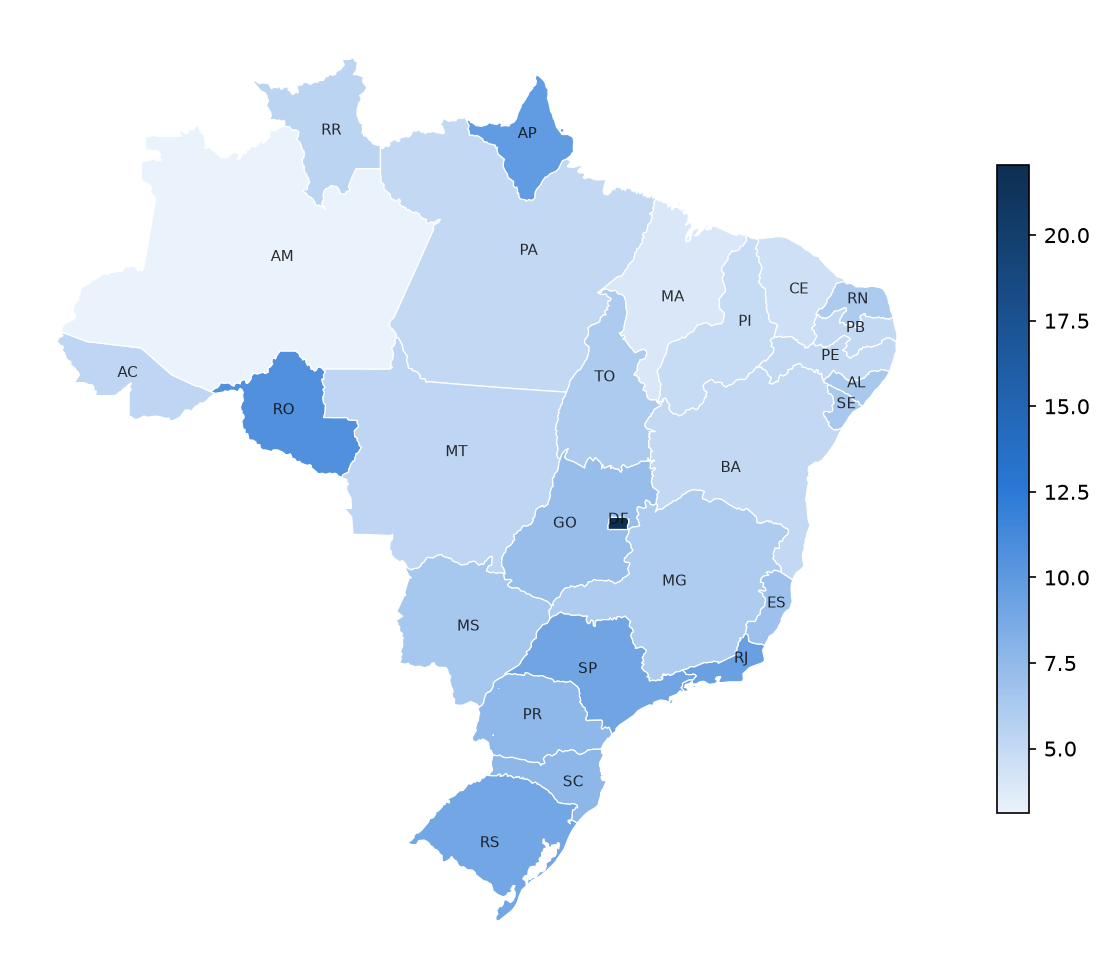
\includegraphics[width=0.7\textwidth]{../figuras/10_mapa_icr_sm_uf.png}
\caption{Average ICR-SM by state, 1995 to 2022. Darker shading indicates a heavier affordability burden.}\label{fig_mapa_icr}
\end{figure}

A second cut, by municipal population size, gives the clearest tariff-burden gradient in the panel (Table~\ref{tab_icr_porte}). The burden rises close to monotonically with size, from a median of 5.7 percent under 5,000 residents to 12.2 percent above 500,000, more than double, even though average water coverage does not follow the same gradient. Because larger municipalities concentrate a larger share of the country's minimum wage workforce, the households most exposed to a heavy burden are disproportionately urban, cutting against a reading of Brazilian water affordability as chiefly a small town problem. Whether this reflects full cost recovery pricing in larger, more autonomous utilities or a more diluted subsidy per connection in denser systems is documented here rather than resolved.

\begin{table}[h]
\caption{Median and mean ICR-SM by municipal population size class}\label{tab_icr_porte}
\centering
\begin{tabular}{@{}lccc@{}}
\toprule
Population size class & Median ICR-SM & Mean ICR-SM & N \\
\midrule
Under 5,000            & 5.7\% & 6.0\%  & 34,041 \\
5,000 to 20,000        & 5.7\% & 6.3\%  & 34,442 \\
20,000 to 50,000       & 7.0\% & 7.5\%  & 11,790 \\
50,000 to 100,000      & 8.2\% & 8.7\%  & 4,801 \\
100,000 to 500,000     & 9.8\% & 10.7\% & 5,066 \\
Above 500,000          & 12.2\% & 13.4\% & 904 \\
\bottomrule
\end{tabular}
\end{table}

\subsection{Planning variables show no robust within municipality association}\label{subsec_resultados2}

In the two way fixed effects model, none of the four lagged planning variables reaches conventional statistical significance (all $p>0.19$). The between $R^2$ reaches 0.85 while the within $R^2$ is close to zero, indicating that year to year movement in these variables carries little of the variation in the tariff burden, which is instead associated with whatever is fixed within a municipality. This is a statement about where the variance sits given the variables the sector reports about itself, not a claim that planning is causally irrelevant under every possible measurement or longer lag structure. The pattern recurs across three alternative lag windows (between $R^2$ 0.85 to 0.87 throughout); only a contemporaneous specification, most exposed to reverse causality, shows significant coefficients, with signs difficult to reconcile with a causal reading from planning to outcome. Full results for all four specifications are in the supplementary material \citep{Figueredo2026Repo}.

This null result is not temporally uniform (Table~\ref{tab_periodo_2012_2022}). The onerous financing share turns significant when the sample is restricted to 2012 onward, with a sign opposite to the original hypothesis, more debt associated with a lighter burden, and investment instability turns significant only under the state income denominator. A plausible reading is that the 2010s included subsidized financing programs for sanitation, so an onerous classification may have captured subsidized credit rather than costly debt; this is reported as an open question about the recent period rather than a resolved exception to the full sample result.

\begin{table}[h]
\caption{Planning variable coefficients with clustered standard errors, dependent variable ICR-SM unless noted}\label{tab_periodo_2012_2022}
\centering
\begin{tabular}{@{}lccc@{}}
\toprule
 & Full sample & 2012--2021 & 2012--2020 \\
 & 2001--2021 & (ICR-SM) & (state income denom.) \\
\midrule
Investment per capita (lag)     & $-0.00002$ & $-0.00002$ & $-0.00003$ \\
                                 & \scriptsize$(0.00004)$ & \scriptsize$(0.00006)$ & \scriptsize$(0.00002)$ \\
Investment instability (lag)    & $-0.015$   & $-0.024$   & $-0.027^{**}$ \\
                                 & \scriptsize$(0.026)$ & \scriptsize$(0.024)$ & \scriptsize$(0.009)$ \\
Onerous financing share (lag)   & $0.035$    & $-0.187^{***}$ & $-0.072^{***}$ \\
                                 & \scriptsize$(0.036)$ & \scriptsize$(0.039)$ & \scriptsize$(0.013)$ \\
Billing loss index (lag)        & $-0.001$   & $-0.0004$  & $0.0001$ \\
                                 & \scriptsize$(0.001)$ & \scriptsize$(0.001)$ & \scriptsize$(0.0003)$ \\
\midrule
$N$              & 41,720 & 29,150 & 25,846 \\
\bottomrule
\end{tabular}
\vspace{2pt}
\footnotesize Standard errors clustered at the municipality level in parentheses. $^{**}p<0.01$, $^{***}p<0.001$. Log municipal population, included as a control in every column, has no valid 2022 observations in this vintage, which removes 2022 from all columns; the state income denominator is further restricted by PNADC availability to 2020.
\end{table}

Two machine learning models, gradient boosting and random forest, were trained to forecast the ICR-SM itself one year ahead, testing the panel finding directly rather than by analogy. Both are outperformed by the naive rule of repeating each municipality's last observed value (MAE 0.54 and 0.56 percentage points respectively, against 0.48 for persistence and 1.97 for a per municipality linear extrapolation), a second, entirely independent empirical route reaching the same substantive conclusion as the panel estimates. Permutation importance shows one partial exception, log GDP per capita, lagged investment per capita, the lagged loss index and investment instability all carry a small positive, non noise contribution, modest but consistent with a weak genuine signal a linear fixed effects specification with a strict one year lag is not positioned to detect. The equivalent forecast for water coverage shows the same qualitative pattern (persistence MAE 2.16 against 3.26 for gradient boosting). Full ablation tables and predicted against observed figures for both outcomes are in the supplementary material \citep{Figueredo2026Repo}.

\subsection{Where a trade off and growth pressure appear}\label{subsec_resultados3}

Interacting coverage with region shows a coverage affordability trade off concentrated in the North and Central West, where coverage gains arrive with a worsening burden, and absent in the Northeast, the region a simple catching up story would predict it most. Population growth reduces water coverage with an economically and statistically meaningful coefficient, while its effect on affordability is not distinguishable from zero; growth in services value added is associated with better, not worse, affordability, plausibly because a larger paying customer base dilutes fixed costs faster than it raises expansion demand. Growth pressure therefore strains access, not price. A model free test, the correlation between each municipality's coverage trend slope and its affordability trend slope, is close to zero, no evidence of a systematic long run trade off between expanding coverage and containing tariffs.

\subsection{Trajectories toward 2033}\label{subsec_resultados5}

A linear extrapolation of historical coverage trends classifies most municipalities as on track for the 99 percent water target by 2033, with a wide regional gap, the South's share projected to miss the target is a fraction of the North's. Sanitation is more precarious, a usable series exists for only 2,971 of 5,549 municipalities, and among municipalities on track for water, the majority are projected to miss the 90 percent sanitation target, coverage of one service carries little information about the other. Validating the coverage projection against a gradient boosting model trained on the same chronological holdout, the machine learning model is outperformed by simple persistence (MAE 2.16 against 3.26 percentage points); the two methods agree on only about a third of municipalities projected to 2033, evidence of sensitivity to forecasting assumptions rather than a defect of either method. Full regional detail and the additional choropleth maps are in the supplementary material \citep{Figueredo2026Repo}.

The same two machine learning models and a linear extrapolation are applied directly to the ICR-SM (Table~\ref{tab_icr_2033}, Figure~\ref{fig_icr_2033}), each starting from every municipality's last observed value, with population growth set to the official IBGE state level projection for 2022 to 2033. The three are reported as separate conditional scenarios rather than averaged into a single estimate, precisely because they disagree in direction, averaging a decline against two increases would manufacture a false consensus, and none is a validated eleven year forecast, the one year ahead validation says nothing about accuracy once a model's own predictions are recursively fed back into itself. The linear scenario continues the gradual decline visible since the mid 2000s, inheriting two decades of real minimum wage appreciation outpacing tariff growth. Both recursive models instead reverse the recent trajectory, by different amounts, gradient boosting fits each new tree to the residuals of the last and extrapolates further, while random forest averages many bootstrapped trees, a form of averaging that pulls recursive forecasts toward a stable point, visible as the random forest trajectory flattening while gradient boosting keeps climbing.

\begin{table}[h]
\caption{National ICR-SM in 2033 under three conditional scenarios}\label{tab_icr_2033}
\centering
\begin{tabular}{@{}lll@{}}
\toprule
Method & National ICR-SM in 2033 & Interpretation \\
\midrule
Linear trend                & 4.5\% & Continuation of historical trajectory \\
Recursive random forest     & 6.0\% & Moderate reversal scenario \\
Recursive gradient boosting & 7.0\% & Sharper reversal scenario \\
\bottomrule
\end{tabular}
\end{table}

\begin{figure}[h]
\centering
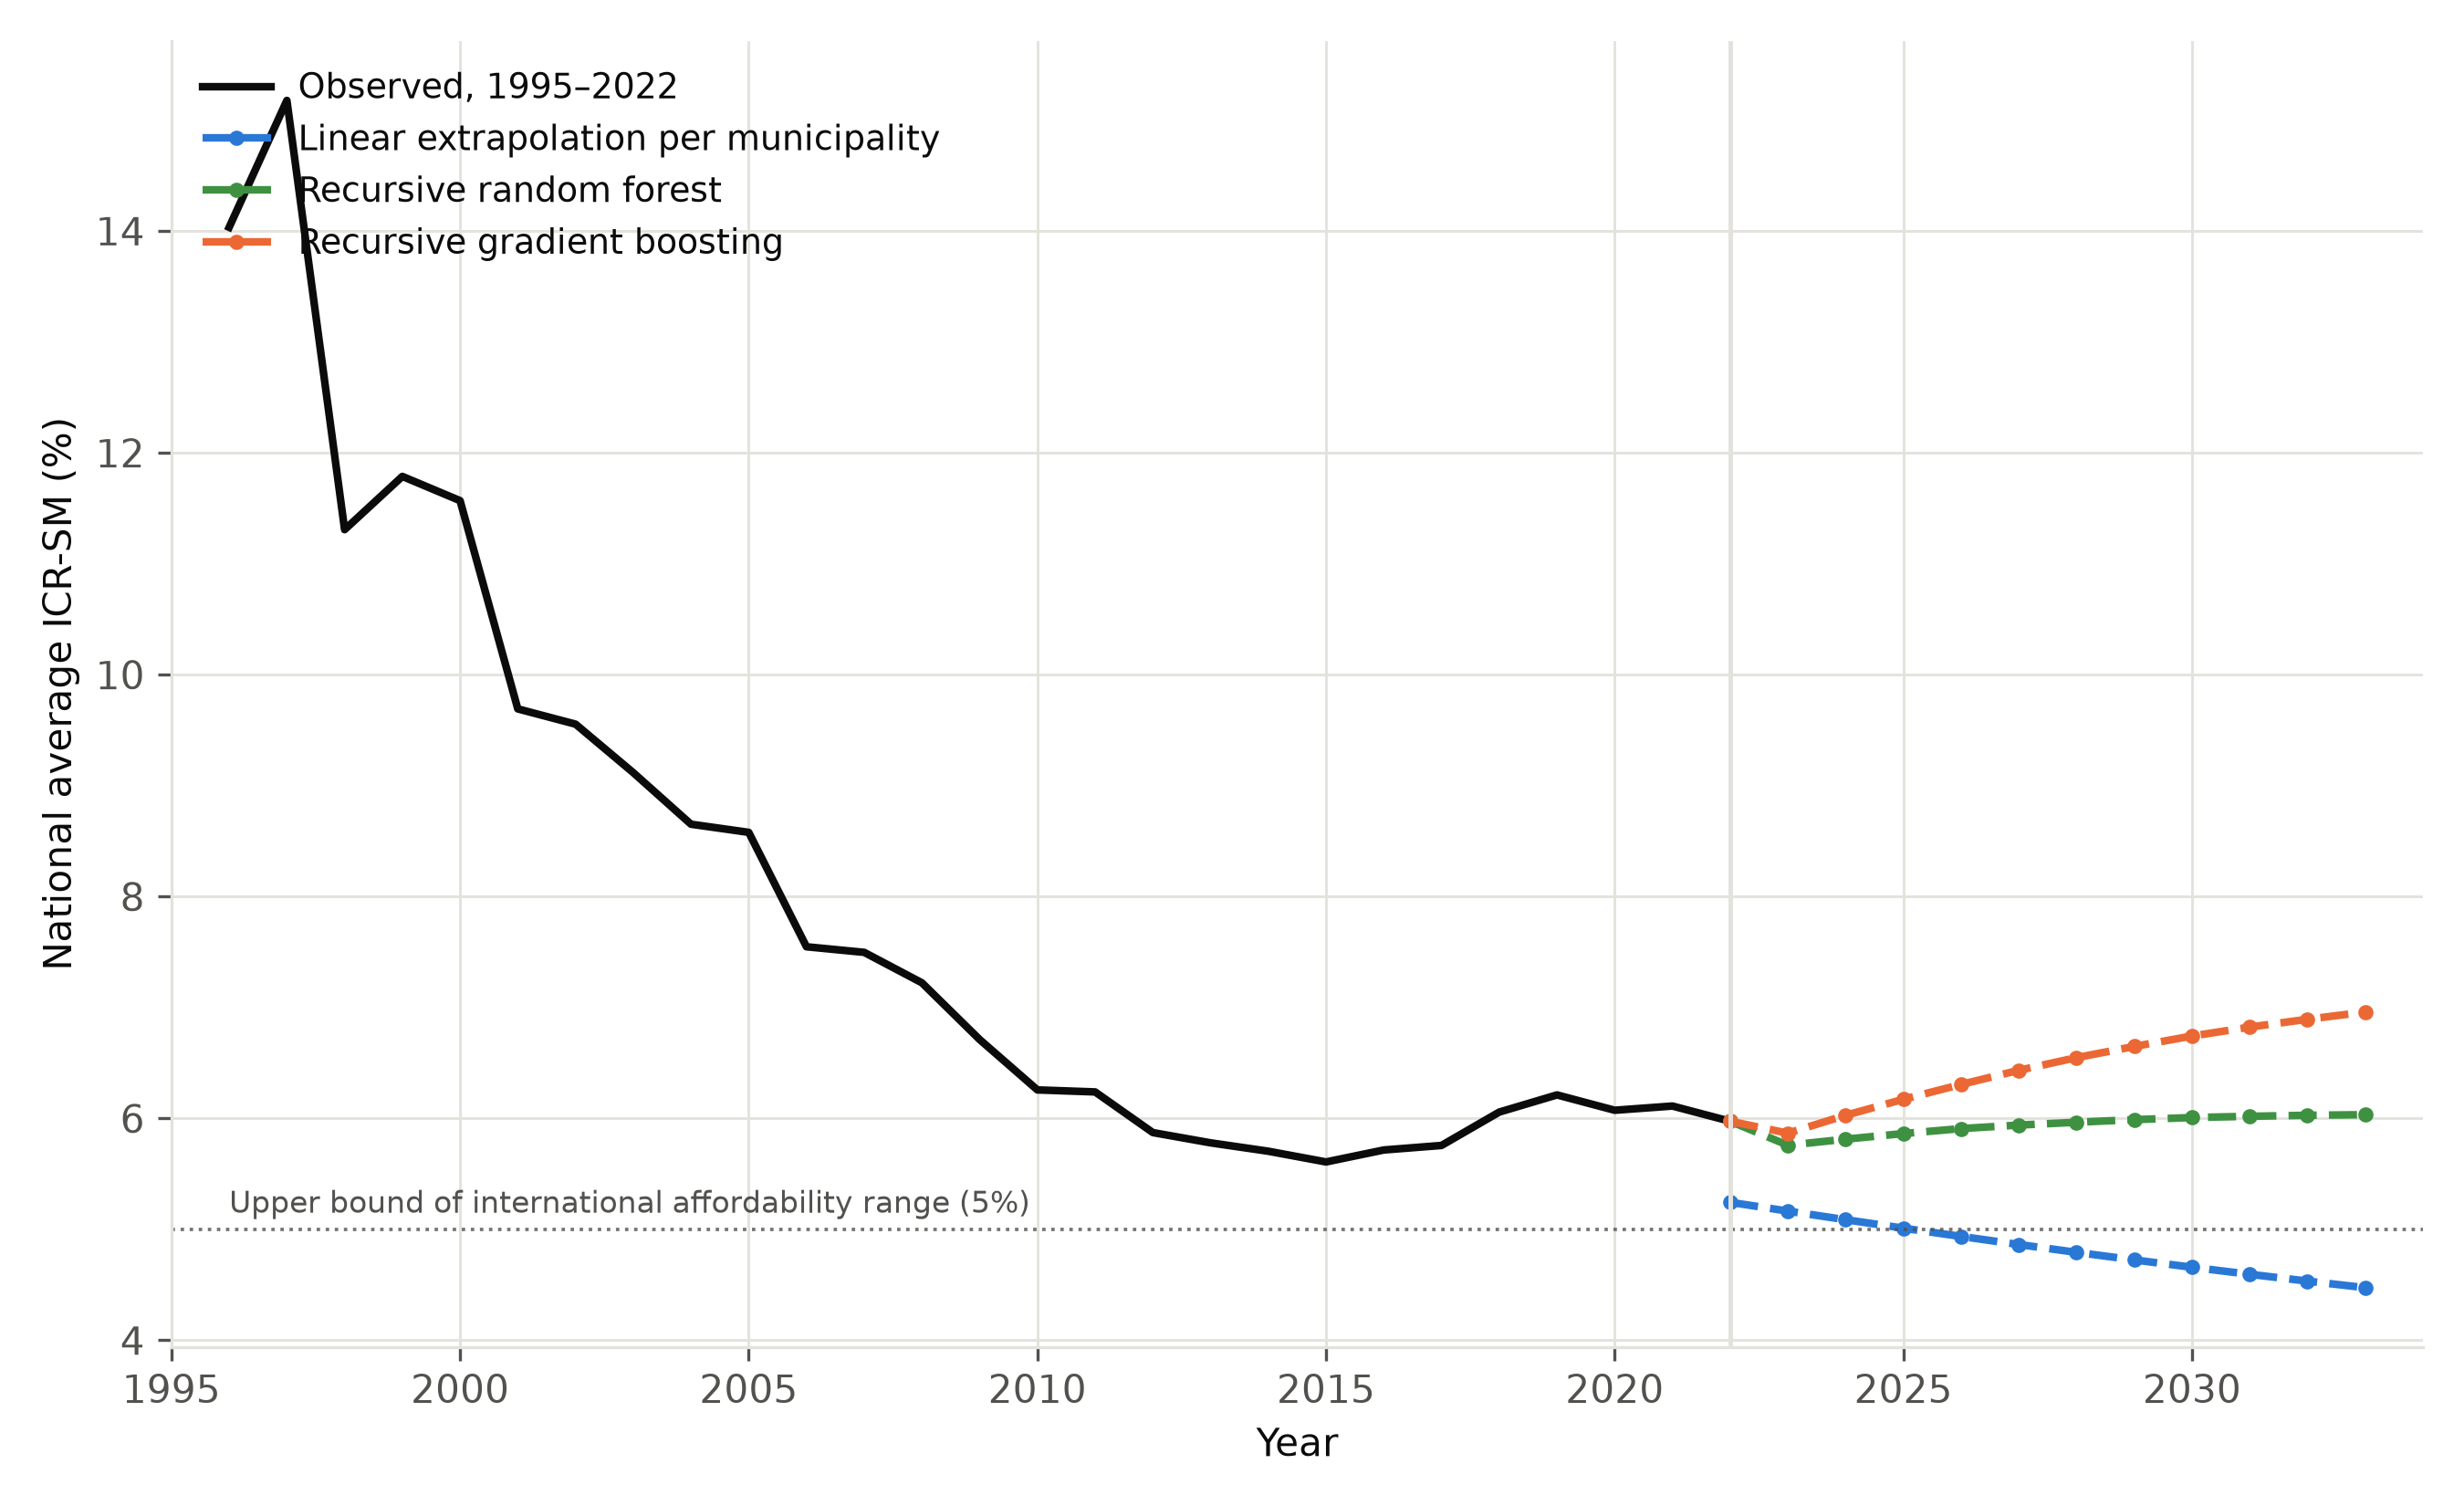
\includegraphics[width=0.8\textwidth]{../figuras/19_projecao_icr_2033.png}
\caption{National average ICR-SM, observed 1995 to 2022 and three conditional scenarios to 2033. None of the three is validated as an eleven year forecast, they are sensitivity scenarios under different assumptions. The dotted line marks the 5 percent upper bound of the international affordability range.}\label{fig_icr_2033}
\end{figure}

None of the three scenarios is put forward as a central estimate or likely range; they are conditional trajectories under different, explicit assumptions, offered to make the uncertainty in any 2033 affordability statement explicit rather than to resolve it. Whether the tariff burden improves or worsens by 2033 depends substantially on a policy variable, the future path of the minimum wage, that lies outside the four planning variables tested here and outside what any of these methods can resolve from the data alone. Taken as a whole, this evidence is more consistent with affordability being shaped by conditions largely fixed within a municipality than with it being moved year to year by the specific planning choices captured in this panel, while coverage remains more sensitive to demographic pressure and carries real forecasting uncertainty, uncertainty that is sharper still, and directional, once the same exercise is applied to affordability itself.

\section{Discussion}\label{sec12}

The evidence assembled above speaks directly to the four questions that motivated this study. Whether affordability responds, within the same municipality, to investment, financing or loss control, the answer across every lagged specification on the full 2001 to 2021 sample is that it does not in any way current statistical power can detect, though this does not hold uniformly, two variables turn significant after 2012, a qualification carried forward rather than set aside. The observed variation is predominantly between municipalities rather than within a municipality over time, and it is that within municipality margin, precisely what a manager can act on from one budget cycle to the next, that the four planning variables account for almost none of. This does not support the premise that affordability is something utilities can be shown to produce through deliberate planning, without establishing the stronger claim that affordability is causally fixed to place, a claim this panel, with its one year lag and four reported variables, is not designed to test. A plausible, though not directly tested, implication is that affordability planning offers a comparatively poor return on managerial attention relative to measurement, which requires no behavioral change; where the actual lever might be, provider governance, technical capacity, longer horizon investment effects or local political economy the SNIS panel does not capture, remains open, and the large between municipality variance is itself an invitation to look there.

The regional and growth results answer the second and third questions. A trade off between expanding coverage and containing tariffs is real but concentrated in the North and Central West, not a national phenomenon, and growth pressure erodes coverage while leaving affordability largely untouched. An equity agenda built around affordability cannot be a single national dial, it needs targeting at the specific regions where price and access genuinely compete and at the specific, demographic rather than financial, pressure coverage is exposed to. The fourth question, whether water and sanitation share a trajectory, receives the least reassuring answer, the two services are close to statistically independent, and a regulatory framework reporting a single universalization date obscures that it tracks two largely unrelated races, one of which is both further behind and measured on a thinner reporting base.

The forecasting exercise adds a dimension most of the affordability literature does not attempt. Two forecasts, identical in architecture and holdout, one for coverage and one for affordability directly, were both outperformed by the simplest conceivable rule, repeating the last observed value; permutation based ablation shows the lagged outcome alone accounts for essentially all predictive accuracy, with one partial exception, GDP per capita and investment level carry a small but genuine signal for affordability that a strictly linear, one year lagged specification is not built to detect. Prediction and estimation, applied to a different outcome and then to affordability directly, reach the same substantive place, the variables this sector reports about its own planning carry little detectable information about either the past or the future. Reporting a projection to a legal deadline without first asking whether any model beats a naive benchmark, largely absent from prior work in this space, is offered here as a minimum bar for future studies that put a date on universal access.

The question this special issue is organized around, what customer equity outcomes look like by the time universal access is due, cannot be answered with a single projected affordability number, and that absence is itself a substantive finding. Extrapolating each municipality's own trend returns the tariff burden inside the international affordability range by 2033; chaining either machine learning model instead reverses the recent improvement, pushing the burden above that range for well over half of municipalities. A 2033 affordability target, if adopted, should be tracked against several explicit, clearly labeled scenarios rather than a single trend line, since the drivers that would move the indicator lie mostly outside what utilities plan and report. None of this argues planning is beyond the reach of policy, only that the planning legible to this sector's information system does not, on this evidence, produce affordability outcomes on a yearly horizon; a national poverty registry matched to this panel, and data on the upfront cost of a new connection, distinct from the ongoing cost measured throughout, are two concrete extensions this information gap motivates.

\section{Conclusion}\label{sec13}

The objective of this study was to test whether the planning levers most often invoked in Brazilian water and sanitation policy explain variation in the tariff burden faced by connected customers over time. Pursued through a municipal panel spanning nearly three decades, with a main estimation sample of 2001 to 2021, and municipality and year fixed effects separating the within municipality margin a manager can act on from the between municipality margin reflecting everything already fixed about a place, the objective was met in the narrow but load bearing sense that none of the four lagged planning variables shows a statistically robust within municipality association with the tariff burden, a result recurring across four alternative specifications and an independent income denominator, while the burden itself rises sharply with municipal size. Two forecasting exercises, a different estimator and a different task, reinforce this reading, gradient boosting could not beat naive persistence for either water coverage or affordability, and permutation importance shows only a small, genuine signal from GDP per capita and investment level, not enough to alter the panel finding.

The remaining three questions were answered along the way. The tariff burden gradient by municipal size, more than doubling from smallest to largest municipalities, is a customer facing equity dimension none of the four planning variables explains and that a future monitoring framework should track directly. A coverage affordability trade off exists only in the North and Central West, growth pressure falls on access rather than price, and water and sanitation follow largely independent trajectories toward 2033, so a combined universalization target risks obscuring real divergence. Projecting the tariff burden to 2033 with a linear extrapolation and two recursive machine learning models produces three scenarios disagreeing in direction, not only magnitude, best treated as an open question about 2033 given how little the tested planning variables explain at an annual horizon.

This account carries limitations that set the agenda for future work. A one year lag rules out same year simultaneity but not reverse causality over a longer horizon; the four planning variables are self reported administrative aggregates, so measurement error works against finding an association even where one exists, and the post 2012 instability is treated as a genuine open question rather than fully resolved. The panel captures only what utilities report to the national information system, so the large between municipality variance remains an unexplained structural residual, and a national poverty registry could test whether local income distribution rather than local planning is what the fixed effects absorb. The affordability measure captures only the ongoing cost of an existing connection, not the upfront cost of obtaining one, and the 2033 forecasts assume historical relationships hold over a horizon more than twice the holdout period used to validate them, a caveat that argues for revisiting every projection as new data become available rather than treating any of them as a fixed answer.

\section*{Acknowledgements}

The authors thank the Coordenacao de Aperfeicoamento de Pessoal de Nivel Superior (CAPES) and the Universidade do Estado da Bahia (UNEB) for their support.

\section*{Data availability}

All source data are publicly available (SNIS, IBGE, Open-Meteo, PNADC); exact access points, the full analysis pipeline (numbered scripts, README, package versions and random seeds), extended robustness tables, permutation importance tables and additional figures not reproduced here are archived as online supplementary material \citep{Figueredo2026Repo}. The constructed municipal panel and other files too large for a code repository are available from the corresponding author upon reasonable request.

\bibliographystyle{elsarticle-num}
\bibliography{../sn-article-template/sn-bibliography}

\end{document}
